\subsection{Bilanzraumkonzept}

%%%%%%%%%%%%%%%%%%%%%%%%%%%%%%%%%%%%%%%%%%%%%%%%%%%%%%%%%%%%%%%%%%%%%%%%%%%%%%%%%%%%%%%%%%%%%%%%%%%%%%%%%%%%%%%%%%%%%%%%%%%%%%%%%%%%%%%%%%%%%%%%%%%%%%%%%%%%%%%%%%%

\subsubsection{System- und Bilanzraumgrenzen}
Eine Bilanz bezieht sich auf das von der Systemgrenze eingeschlossene Kontrollgebiet (\cite[Kapitel 1.5]{Ahrendts.2014}). 
Die Systemgrenze kann dabei unter Berücksichtigung der Zweckmäßigkeit frei definiert werden (\cite[Kapitel 1.5]{Ahrendts.2014}).
Die Berechnung der in einen Bilanzraum ein- und austretenden Ströme wird als Bilanzierung bezeichnet (\cite[S. 65]{Rönsch.2015}).
Folglich kann das thermodynamische System welches von Ahrendts (2014) und Rönsch (2015) beschrieben wurde durch das Konzepts: 
Bilanzraum abstrahiert und dargestellt werden. 

Einen Ansatz zur Definition von Bilanzräumen liefert Miller (2016, S. 105) mit der Konkretisierung von Bewertungsräumen mittels Kriterien der Bilanzgrenze, dem 
Aggregationsniveau und der Bewertungseinheit. 
Das definierte System dient der Bewertung der Nutzung der Ressourcen, und bewertet die Effizienz (vgl. Gleichung \eqref{EffizienzgleichungMiller}) eines Systems 
(\cite[S. 107]{Miller.2016}).

\begin{equation}
    \text{Effizienz} := \frac{\text{Erreichter Nutzen}}{\text{Aufwand}}
    \label{EffizienzgleichungMiller}
\end{equation}

Der Aufwand umfasst nach Miller (2016, S. 108f.) unterschiedliche Ressourcen. 
Im Kontext energiewirtschaftlicher Fragestellungen liegt der Fokus auf der Ressource Energie (\cite[S. 108f.]{Miller.2016}).
Der Nutzen ist vom Untersuchungsgegenstand abhängig und wird im Kontext der energiewirtschaftlichen Fragestellung häufig über Energiedienstleistungen operationalisiert (\cite[S. 107]{Miller.2016}). 
Die befriedung des Nutzens impliziert einen entstehenden Nutzenergiebedarf zur erfüllung der Energiedienstleistung (\cite[S. 107]{Miller.2016}).
Sowohl die Ressourcen des Aufwands als auch die Energiedienstleistung auf der Nutzenseite werden durch eine Bewertungseinheit formalisiert (\cite{Miller.2016}).
Die in \eqref{EffizienzgleichungMiller} aufgestellte Nutzen-Aufwand-Relation stellt die Grundlage der Definition der Bilanzraumgrenze dar.
Die Bilanzraumgrenze lässt sich somit in die aufwandsseitige Bilanzgrenze, die alle zu bilanzierenden Ressourcen umfasst, und die nutzenseitige Bilanzgrenze, 
die sich auf die zu bilanzierende Energiedienstleistung bezieht (\cite[S. 111]{Miller.2016}).

Das von Miller (2016) beschriebene Konzept zeigt eine weitere Perspektive auf die in \eqref{BilanzierungsgleichungAhrendt} und \eqref{BilanzierungsgleichungAhrendtStrom} 
formalisierte Bilanzierung. 
Sie betrachtet die Energieeffizienz des durch die Bilanzgrenzen eingeschlossenen Bewertungsraums und teilt eine Bilanz in Aufwands- und Nutzenseite.
Aufwandsseitig sind die in \eqref{BilanzierungsgleichungAhrendt} zufließenden Ströme, also die dem System zugeführten Ressourcen der Zustandsgröße, zu betrachten.
Nutzenseitig müssen abfließende Ströme betrachtet werden. Die abfließenden Ströme werden durch den Nutzenergiebedarf zur befriedigung einer Energiedienstleistung 
repräsentiert. 

%%%%%%%%%%%%%%%%%%%%%%%%%%%%%%%%%%%%%%%%%%%%%%%%%%%%%%%%%%%%%%%%%%%%%%%%%%%%%%%%%%%%%%%%%%%%%%%%%%%%%%%%%%%%%%%%%%%%%%%%%%%%%%%%%%%%%%%%%%%%%%%%%%%%%%%%%%%%%%%%%%%

\subsubsection{Untersuchungsgegenstand und Nutzengrößen}

Der Untersuchungsgegenstand ist von Zentraler bedeutung im von Miller (2016) beschrieben Konzept: Bewertungsräume.
Auf Grundlage des Untersuchungsgegenstands ist eine Auswahl angemessener Nutzengrößen mit entsprechenden Bewertungseinheiten notwendig.
Da auch die Definition der Systemgrenze vom Untersuchungsgegenstand beeinflusst wird (\cite[S. 109]{Miller.2016}), gilt die Zweckmäßigkeit der Systemgrenze auch für die 
zu untersuchenden Nutzengrößen.
Die DIN EN ISO 50001:2018-12 gibt mit dem Ziel der fortlaufenden Verbesserung der energiebezogenen Leistung eine  Vorgabe zur zweckmäßigen Definition 
der Nutzengrößen (\cite[S. 11]{DIN50001.2018}).
Die Vornorm DIN V 18599-1:2018-09, herausgegeben vom Deutschen Institut für Normung e. V. (2018, S. 1), behandelt die energetische Bewertung von Gebäuden und stellt ein 
Verfahren zur Durchführung der Gesamtenergiebilanz des Untersuchungsgegenstands: Gebäude bereit (\cite[S. 9]{DIN18599.2018}). 
Die Vornorm betrachtet neben dem Gebäude auch Gebäudezonen als Untersuchungsgegenstände (\cite{DIN18599.2018}).
Der Untersuchungsgegenstand der Norm und ihre Ausrichtung auf die energetische Bewertung erfüllt folglich die Zweckmäßigkeit hinsichtlich der Anwendung in 
Organisationen des tertiären Wirtschaftssektors und der DIN EN ISO 50001:2018-12. 

Im Rahmen der energetischen Bewertung von Gebäuden betrachtet die DIN V 18599-1:2018-09 die Bilanzierung des Nutz-, End- und Primärenergiebedarfs (\cite{DIN18599.2018}).
Das von Miller (2016) entworfene Konzept legt seinen Fokus auf den Nutzenergiebedarf.
Die Vornorm definiert die Heizung, Kühlung, Lüftung, Trinkwarmwasseraufbereitung und Beleuchtung von Gebäuden oder Gebäudezonen 
als relevante Energiedienstleistungen zur energetischen Bewertung von Gebäuden (\cite{DIN18599.2018}).
Im Rahmen der Vornorm wird der Nutzenergiebedarf als Überbegriff für Nutzwärmebedarf, Nutzkältebedarf, Nutzenergiebedarf für Trinkwarmwasser, 
Beleuchtung und Befeuchtung definiert (\cite[Kapitel 3.1.3]{DIN18599.2018}).
Der durch eine Energiedienstleistung entshende Nutzenergiebedarf muss durch Energiemengen gedeckt werden, welche von der DIN V 18599-1:2018-09 in 
abhängigkeit zur Energiedienstleistung wie folgt definiert wird.

\begin{itemize}
    \item \textbf{Nutzenergie für Beleuchtung}: Die Energiemenge, die zur Ausreichenden Beleuchtung des Gebäudes beziehungsweise der Gebäudezone 
    aufgewendet werden muss (\cite[Kapitel 5.3.1]{DIN18599.2018}).
    \item \textbf{Wärmeenergie}: Die Wärmemenge, die dem Gebäude beziehungsweise der Gebäudezone zusätzlich (bedarfs-)geregelt zugeführt wird, 
    um die vorgegebene Sollinnentemperatur einzuhalten (\cite[Kapitel 5.3.1]{DIN18599.2018}).
    \item \textbf{Kälteenergie}: Die Kälteeinträge, die dem Gebäude bzw. der Gebäudezone zusätzlich (bedarfs-)geregelt zugeführt werden, um die 
    vorgegebene Sollinnentemperatur einzuhalten (\cite[Kapitel 5.3.1]{DIN18599.2018}).
    \item \textbf{Nutzenergie für die Trinkwarmwasserbereitung}: Die Energiemenge, die zum Erwärmen, Kühlen, Befeuchten und Entfeuchten der 
    Luft in einer raumlufttechnischen Anlage zu- bzw. abgeführt werden muss, um den erforderlichen Zuluftzustand zu erreichen (\cite[Kapitel 5.3.1]{DIN18599.2018}).
    \item \textbf{Nutzenergie für die Luftaufbereitung}: Die Energiemenge, die zum Erwärmen, Kühlen, Befeuchten und Entfeuchten der Luft in 
    einer raumlufttechnischen Anlage zu- bzw. abgeführt werden muss, um den erforderlichen Zuluftzustand zu erreichen (\cite[Kapitel 5.3.1]{DIN18599.2018}).
\end{itemize}


\begin{figure}[H]
    \centering
    \includegraphics[width=1\textwidth]{../../Ressourcen/Abbildungen/Energiewertschöpfingskette_Posch.jpg}
    \caption{Energiewertschöpfungskette. (Dargestellt von Posch (2011, S. 45))}
    \label{fig:Energieflussschema_Posch}
\end{figure}

Die in Abbildung \eqref{fig:Energieflussschema_Posch} visualisierte Energiewertschöpfungskette, ordnet die Nutzenergie als Energieform die aus der umwandlung von Endenergie 
in einen Energieträger der Nutzenergie zur erfüllung von Energiedienstleistungen dient, ein.
Da die Endenergie die Energiemenge ist, die dem Bilanzraum zur bestimmungsgemäßen Nutzung bereitgestellt wird (\cite[Kapitel 3.1.2]{DIN18599.2018}), 
deckt diese Energieform die Energiemenge der Ressourcen auf der Aufwandsseite der Bilanzierung nach Miller (2016).
Folglich muss der nutzenseitige Nutzenergiebedarf, welcher durch die befriedigung von Energiedienstleistungen entsteht durch die aufwandsseitige Endenergie gedeckt werden.
Bei der Umwandlung der Energieformen sind die in Abblidung \eqref{fig:Energieflussschema_Posch} dargestellten Umwandlungs- und Transportverluste zu beachten.


Abbildung \eqref{fig:Übersicht_Bilanzräume} ordnet die mithilfe der DIN V 18599-1:2018-09 erfassten Nutzengrößen des Untersuchungsgegenstands in das von 
Miller (2016) erarbeitete Konzept der Bewertungsräume ein und erweitert dieses um den Einfluss der Endenergie.

\begin{figure}[H]
    \centering
    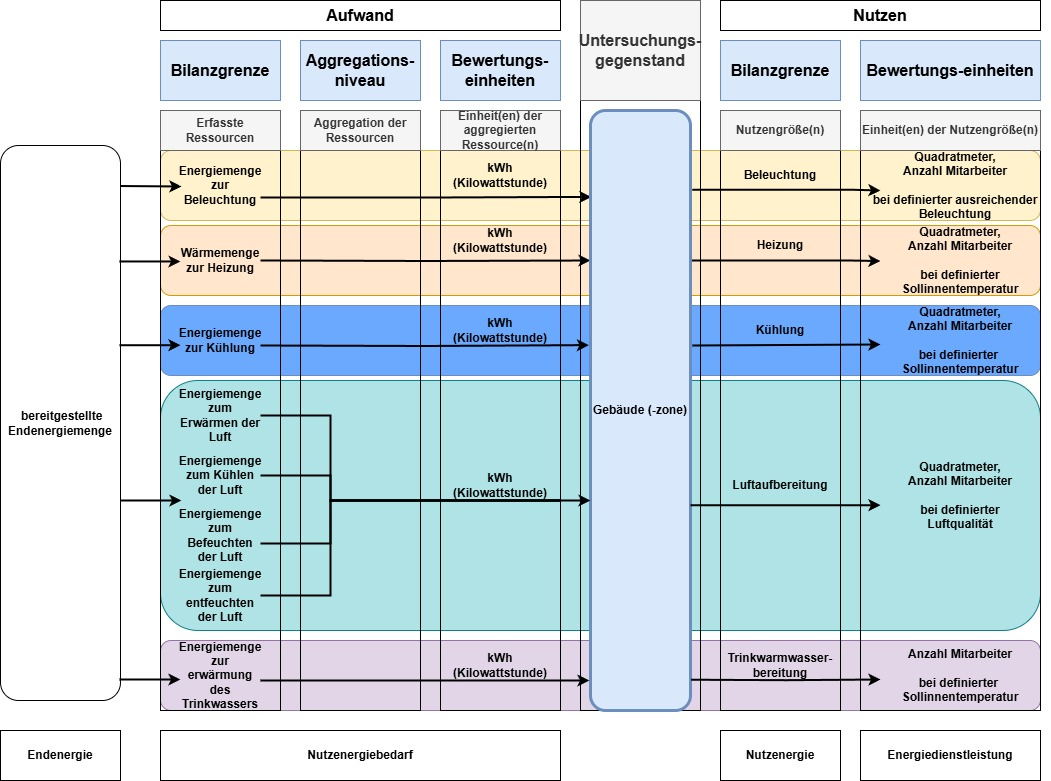
\includegraphics[width=1\textwidth]{../../Ressourcen/Abbildungen/Nutzengröße_Bewertungseinheit.jpg}
    \caption{Bilanzgrenzen Aufwandsseitig/Nutzenseitig. (Eigene Darstellung basierend auf Miller (2016) und DIN V 18599-1:2018-09 (2018))}
    \label{fig:Übersicht_Bilanzräume}
\end{figure}

%%%%%%%%%%%%%%%%%%%%%%%%%%%%%%%%%%%%%%%%%%%%%%%%%%%%%%%%%%%%%%%%%%%%%%%%%%%%%%%%%%%%%%%%%%%%%%%%%%%%%%%%%%%%%%%%%%%%%%%%%%%%%%%%%%%%%%%%%%%%%%%%%%%%%%%%%%%%%%%%%%%

\subsubsection{Energieströme und Bewertungseinheiten}

In Gleichung \eqref{BilanzierungsgleichungAhrendt} wird zwischen zu- und abfließenden Energieströmen des Systems unterschieden.
Im in Abbildung \eqref{fig:Übersicht_Bilanzräume} visualisierten Bilanzraumkonzept bilden die über die Bilanzgrenze zuströmenden Endenergiemengen 
zur deckung des Nutzenergiebedarfs die zufließenden Energieströme ab. 
Diese Energiemengen werden nach dem Konzept von Miller (2016) durch die aufwandsseitigen Ressourcen zur befriedigung der Dienstleistungen erfasst.
Aufwandsseitige Ressourcen können zu einer Ressource mit einer Bewertungseinheit zusammengefasst werden (\cite[S. 112]{Miller.2016}).  
Die zufließenden Energieströme werden mit der Bewertungseinheit: kWh und deren Vielfachem bilanziert, da diese Einheit bei Energiebilanzen in der Regel 
für alle Energieformen bevorzugt verwendet wird (\cite[S. 65]{Konstantin.2023}).

Im Bilanzraumkonzept der Abbildung \eqref{fig:Übersicht_Bilanzräume} werden die abfließenden Energieströme durch die befriedigte Energiedienstleistung abgebildet.
Da eine Energiedienstleistung nicht als Energiemenge erfasst werden kann, ist eine Konkretisierung der Energiedienstleistung durch eine angemessene Bewertungseinheit, 
welche vom Untersuchungsgegenstand impliziert wird, notwendig (\cite{Miller.2016}). 
Diese Bewertungseinheit ist keine Energieeinheit und kann beispielsweise bei der Untersuchung der Temperierung 
von Räumen die Quadratmeteranzahl des Bilanzraums bei einer definierten Soll-Temperierung sein (\cite{Miller.2016}). 

%%%%%%%%%%%%%%%%%%%%%%%%%%%%%%%%%%%%%%%%%%%%%%%%%%%%%%%%%%%%%%%%%%%%%%%%%%%%%%%%%%%%%%%%%%%%%%%%%%%%%%%%%%%%%%%%%%%%%%%%%%%%%%%%%%%%%%%%%%%%%%%%%%%%%%%%%%%%%%%%%%%

\subsubsection{Energiequellen und -senken}
Gleichung \eqref{BilanzierungsgleichungAhrendt} unterscheidet neben zu- und abfließenden Energieströmen auch zwischen Energiequellen und -senken.
Quell- und Senkenströme treten in einer Energiebilanz nach dem ersten Hauptsatz der Thermodynamik nicht auf, da Energie eine Erhaltungsgröße ist (\cite[S. 14]{Ahrendts.2014}).
Im Rahmen der DIN EN ISO 50001:2018-12 bezieht sich der Begriff "Energie" auf verschiedene Arten von Energie, die erworben, gespeichert, aufbereitet, in einer Einrichtung oder einem Prozess verwendet
oder zurückgewonnen werden können (\cite[Kapitel 3.5.1]{DIN50001.2018}). 
Energie kann im Rahmen der Norm als Elektrizität, Brennstoff, Dampf, Wärme, Druckluft oder vergleichbares Medium auftreten (\cite[Kapitel 3.5.1]{DIN50001.2018}).
Folglich können alle Energieströme, in denen Energie in eine Energieform umgewandelt wird, die nicht die genannten Kriterien erfüllt, als Energiesenken betrachtet werden.
Analog dazu können alle Energieströme, bei denen Energie, die nicht den von der Norm aufgestellten Kriterien entspricht, in eine nach ISO 50001 definierte Energieform
umgewandelt wird, als Energiequellen betrachtet werden.
In der Praxis stellen die in Abbildung \eqref{fig:Energieflussschema_Posch} dargestellten Umwandlungs- und Transportverluste Energiesenken dar. 
Energiequellen können beispielsweise
PV-Anlagen sein, da diese die Energie des Sonnenlichts, welche im Rahmen der DIN EN ISO 50001:2018-12 nicht als Energiemedium betrachtet wird, in für die Organisation 
nutzbare Endenergie in Form von Elektrizität umwandeln und zur Verfügung stellen.

\subsubsection{Bilanzraumstrukturen}
Bisher wurde die strukturelle Definition von Bilanzräumen unter Berücksichtigung praktischer Herausforderungen gemäß der DIN EN ISO 50001:2018-12 in Organisationen 
des tertiären Wirtschaftssektors betrachtet. 
Eine Betrachtung der Beziehungen zwischen Bilanzräumen, beziehungsweise deren Hierarchie weist auch eine Relevanz zur Erfüllung der DIN EN ISO 50001:2018-12 auf.
So kann ein Bilanzraum in mehrere Teilbilanzräume zerlegt werden (\cite[S. 310]{Engelmann.2015}). 
Dies kann durch die Disaggregation in einzelne Prozesse, Anlagen oder räumlich getrennte Bereiche realisiert werden (\cite[S. 310]{Engelmann.2015}), 
wobei die Disaggregation in Prozesse bei Organisationen des tertiären Wirtschaftssektors, aufgrund der niedrigen Energielast für Prozesse (vgl. Abbildung \eqref{fig:Energieverbrauch_Wärme_DE}), 
eine geringere Relevanz hat.
Analog zur Zerlegbarkeit eines Bilanzraums lässt sich auch der Untersuchungsgegenstand eines Bilanzraums hierarchisch aufgliedern (\cite[S. 109]{Miller.2016}).
Die in Abbildung \eqref{fig:Übersicht_Bilanzräume} dargestellten Bilanzgrenzen für den Untersuchungsgegenstand Gebäude können also folglich in räumlich getrennte 
Gebäudezonen, wie zum Beispiel Etagen oder Räume, zerlegt werden (vgl. Abbildung \eqref{fig:Disagggregation_Bilanzraum_Untersuchungsgegenstand}).

\begin{figure}[H]
    \centering
    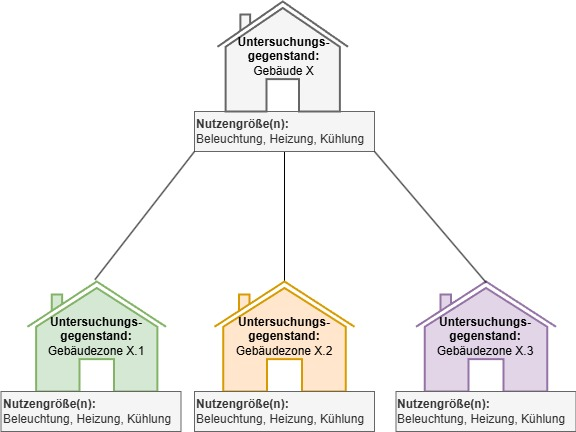
\includegraphics[width=0.63\textwidth]{../../Ressourcen/Abbildungen/Untersuchungsgegenstand_Zerlegt.jpg}
    \caption{Disagggregation eines Untersuchungsgegenstands. (Eigene Darstellung)}
    \label{fig:Disagggregation_Bilanzraum_Untersuchungsgegenstand}
\end{figure}

Zur Erfassung der Energiedaten einer Organisation bedarf es einer detaillierten und aussagekräftigen Analyse der Unterscheidung nach Verbrauchsarten 
(\cite[S. 14]{Hohnhold.2013}). Dabei ist die Disaggregation der Daten von der Größe der Organisation und dem Zweck der Analyse abhängig (\cite[S. 14f.]{Hohnhold.2013}).
Zur Analyse der Verbrauchsarten kann es also auch sinnvoll sein, Bilanzräume anhand ihrer definierten Nutzengrößen zu disaggregieren.
In \eqref{fig:Disagggregation_Bilanzraum_Nutzengrößen} ist ein Beispiel für eine Disaggregation nach Nutzengrößen 
zur Analyse der Unterscheidung nach Verbrauchsarten visualisiert.

\begin{figure}[H]
    \centering
    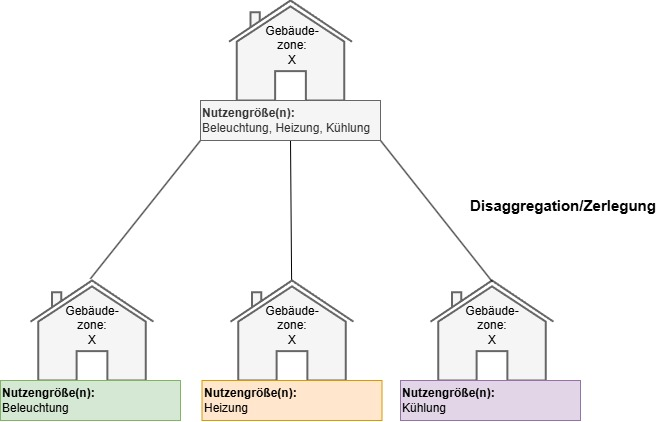
\includegraphics[width=0.63\textwidth]{../../Ressourcen/Abbildungen/Nutzengröße_Bewertungseinheit_Zerlegt.jpg}
    \caption{Disagggregation eines Bilanzraums nach Nutzengrößen. (Eigene Darstellung)}
    \label{fig:Disagggregation_Bilanzraum_Nutzengrößen}
\end{figure}